% !Tex root = dis.tex
\chapter{Literature Review}
\graphicspath{{./images/ch2/}}

In the introduction, I gave a high level overview of software engineering and cognitive load theory and the origins of the fields. In this section, I start by reviewing the literature of software engineering and computer science as it has related to specific attempts to influence the practice of programming. Software engineering research covers a space as disparate as processes surrounding the elicitation of software requirements, visualization techniques for software designs, estimation practices for predicting delivery cycles, probabilistic testing, and more.  I viewed CLT specifically from the frame of how it can influence the practice and understanding of programming. I progress chronologically, looking at specific programming recommendations of the 1970s and 1980s and moving towards the 2000s and 2010. I also review the way computer science has attempted to quantify the concept of complexity in computer programs through the development of metrics. I find that although CLT is neither directly invoked nor indirectly referenced, much of the modern practitioner literature of Agile Software Development and Software Craftsmanship \cite{McBreen2001} extensively focus on the comprehensibility of computer programs. The practices and principles proposed in these works have conceptual similarity to cognitive load theory. By the end of this section, the reader should have a sense of established research that is similar to mine in software engineering and a high-level overview of cognitive load theory.


Others have attempted to improve programming practice in the past. Edsgar Djikstra published the provocative \textit{Go To Statement Considered Harmful} \cite{Dijkstra1968} in a letter to the editor of Communications of the ACM in 1968. This paper, premised with the assertion that the ``the quality of programmers is a decreasing function of the density of go to statements in the programs they produce'' essentially helped launch the conversation that “the way you write code matters” by arguing that one particular tool in high level programming languages, the goto statement, made programs harder to understand.  Djikstra continued refining these ideas and published a set of notes which led to a book on Structured Programming \cite{Dijkstra1972}.  Structured Programming prescribed the use of control structures-- such as if/else statements, cases, and looping statements--instead of only variable assignment statements and jumps to labeled sections.  Structured Programming influenced the development of new programming languages like Kernighan and Ritchie’s C Programming Language \cite{Kerninghan1988}, which incorporated control structures as the fundamental primitives of writing code. Structured programming triggered the elaboration of programming paradigms as diverse as imperative programming, procedural programming, and object-oriented programming. Imperative programming simply arranges program statements in order of execution, very similar to writing a task list. Procedural programming organizes imperative code into subroutines, named groups of imperative statements that can form a basis for abstraction and apply Parnas principle of information hiding \cite{Parnas1972}. Object-oriented programming defines systems in terms of message passing between independent units that encapsulate data and the operations on that data called objects \cite{Kay1993}. In a parallel track, Donald Knuth developed Literate Programming \cite{Knuth1992,Knuth1984}. Programmers who write in a “literate” style combine prose and narrative to elaborate the function of the application. The author of a literate program writes with readability and comprehensibility in mind as a direct consequence of the formulations in accompanying text. Literate Programming has yet to penetrate the majority of the programming zeitgeist, remaining a fairly niche research interest. Nevertheless, many authors have experimented with it and reported enhanced clarity \cite{Ramsey1994}. There are many other paradigms of programming, as have been extensively collected and classified by Van Roy [67]. All of these paradigms seek to apply a specific set of constraints and models of interaction to computer programs to make it easier for a programmer to reason about and implement their design. Some researchers have looked at the potential cognitive elements of programming paradigms \cite{White2005,Kim1992.Rosson1990}, others have looked at cognitive elements independently of programming paradigm \cite{Douce2008}, but the discipline lacks a de facto standard for the evaluation of the cognitive impact of programming paradigm.


Rather than measure complexity through the impact on human cognition directly, Software metrics comprise effort by the software engineering research community to quantify the results of the software process. The original, most cited software metric is the Line of Code (LOC) and the analogous KLOC (thousands of lines of code). An oft-maligned metric— that does not account for the internal complexity or structure of a program— LOC has nonetheless remained common due to simplicity of measurement. Attempts to provide more information about the inner working of a program have led to the creation of metrics such as Halstead’s Software Science \cite{Halstead1977}, McCabe’s Cyclomatic Complexity \cite{McCabe1976}, and Albrecht’s Function Points \cite{Albrecht1983}. These approaches have found limited success. Empirical studies have produced very little conclusive evidence as to the efficacy of these metrics \cite{Curtis1980}, with many equivocal examples \cite{Curtis1984}. Modern metrics research, however, is attempting to incorporate elements of cognitive science into the art of understanding software.  Wang’s study of the cognitive complexity of software serves as a bridge for the metrics work into this world \cite{Wang2009} \cite{Shao2003}. Wang develops a set of meta-cognitive models for the description and understanding of computer programs, then constructs a set of experiments that compare and contrast the cognitive complexity of different constructs. The argument is that the metrics generated through such analysis are more accurate descriptors of software complexity than symbolic, structural, or functional complexity metrics. 


Cognitive metrics for software scratches the surface of what cognitive science can offer computer science and software engineering. Software maintainers spend more time reading code than they do writing new code. Many developers who write new code often find themselves working with unfamiliar technologies or in an unfamiliar domain. People commonly believe there are similarities between programming and education, but no unifying link in theory has tied successful programming outcomes to established educational theory.  One such relevant theory is Cognitive Load Theory \cite{Clark2006}, which informs the way educational designers seek to develop curricular materials. Human Computer Interface (HCI) designers leverage it to provide better user experiences \cite{Hollender2010,Oviatt2006}. Nevertheless, programmers have not applied this work towards actually changing the way they write code for other programmers. Software engineering research has been focused on other areas.


Software Engineering literature of the early 1990s continued the work of the 1980s in software processes and modeling, leading to the development of the Unified Modeling Language (UML) \cite{Rumbaugh1999}] and the associated Rational Unified Process (RUP) \cite{Jacobson1999}. In 1994, the Gang of Four published their seminal Design Patterns \cite{Gamma1994} catalog, a hybrid design/architecture and implementation publication that inspired a rush of patterns oriented research activity in the community, including implementation patterns \cite{Kent2007}, testing patterns \cite{Beck2002}, enterprise application architecture patterns \cite{Fowler2002}, language implementation patterns \cite{Parr2010}, and others. In February 2001, a group of experienced and well-respected software engineers published the Agile Manifesto \cite{Beck2001}. A counterpoint to RUP, agile software development emphasized less documentation, tools, and repeatable processes. Instead, it championed greater emphasis on relationship building and collaboration. This approach quickly became popular with industry, especially with the rise of web application development. Its emphasis on results effectively captured the spirit of the rise of the Internet and fast-paced nature of web development. Consequently, an explosion of interest for effective ways of organizing and managing agile software teams led to the development of models such as Extreme Programming \cite{Beck1999,Rising2000}, and Kanban \cite{Anderson2010}.


Many of the forerunners of Agile were leading evolution in multiple areas of software engineering. Andrew Hunt and Dave Thomas wrote The Pragmatic Programmer \cite{Hunt2010}, fleshing out the baseline principles of the Agile Manifesto into a programming philosophy built on pragmatism. Kent Beck helped elaborate Extreme Programming \cite{Beck1999}, codified best practice Implementation Patterns \cite{Kent2007}, and wrote the most popular Java variant of the xUnit testing framework, JUnit, as part of his work in proselytizing Test-Driven Development \cite{Beck2002}. Martin Fowler developed a widely regarded Refactoring patterns catalog \cite{Fowler1999} extending from Bill Opdike’s PhD thesis \cite{Opdyke1992} to provide a structured, behavior-preserving methodology for modifying existing code to promote clarity and reuse. Robert C. Martin helped expound some basic principles that have become the bedrock of SOLID object-oriented software development \cite{Martin2002}, including the Single Responsibility Principle, the Interface Segregation Principle, and Dependency Inversion alongside Barbara Liskov’s Substitution Principle \cite{Liskov1987} and Bertrand Meyer’s Open/Closed Principle \cite{Meyer1997}.


These industrial contributions have ironically transformed much of the software engineering landscape—particularly in web and mobile software development, the preeminent paradigms of the 21st century—at arguably a broader scale than academic software engineering research. Recognition of this dichotomy between the research emphasis and industrial literature has fueled the rise of the Software Craftsmanship movement \cite{McBreen2001}. Software Craftsmanship espouses treating programming as a craft more than a science or an engineering discipline. In such epistemology, dedicated artisans construct the best software. Such artisans hone their craft through discipline, practice, and apprenticeship/journeyman style interactions with masters.


One could see Software Craftsmanship as a reaction against and rejection of Software Engineering. It eschews the emphasis on process, models, and up-front work to build software systems. Alternately, one could argue that it represents a competing school of thought. Much like Cubism and Expressionism were competing schools of thought in 20th century painting, software craftsmanship and SWEBOK \cite{Abran2001} [56]  based approaches may be seen as competing schools of thought within 21st century software engineering. One can relate this to the difference shown in DeRemer and Kron’s "Programming-in-the large versus programming-in-the-small" \cite{DeRemer1975}. Many software craftsmen seek to apply cognitive science to improve their craft. Andy Hunt wrote a book to help programmers “refactor their wetware” by applying concepts from cognitive science \cite{Hunt2008}. They have yet to link cognitive science to writing code. CLT is the link.

\section{Establishing the link between Cognitive Load Theory and Software Engineering through Software Craftsmanship}

Before I dive into the conceptual overlap between software craftsmanship best practices and CLT, it will be helpful to define the concepts individually. I begin by outlining concepts from software craftsmanship, then defining concepts from CLT, then describing their connection.

The Single Responsibility Principle states that “a class should have only one reason to change.” \cite{Martin2002} For example, the design of a vending machine class may include methods to add money, vend a product, set the prices of individual products, restock individual products, and refund money. If the currency of the machine has to change, the implementation may need to be modified. If the product stocking needs to support batches, the implementation may need to be modified. This design conflates inventory management with price calculation. A Single Responsibility Principle-based design would break apart the functionality such that the vending machine has an inventory and a cost calculator. Application of the SRP tends to break larger objects into smaller, more cohesive objects. This increased cohesion is reminiscent of the cognitive concepts of chunking, essentially the SRP calls for smaller, independent chunks. It also aligns with CLT guidelines of paring content down to essentials and writing high coherent text for low-knowledge learners.

\subsection{Open-Closed Principle}

The Open-Closed Principle states that software entities should be open for extension but closed for modification \cite{Martin2002}. This seemingly unachievable goal drives designs towards simple abstractions that change rarely but can add behaviors to a system through different implementations. For example, an online retailer may select the right hello message to display on a landing page based on the country the customer is in based on a Greeter class. If that class uses a hardcoded array, whenever that retailer expands to a new country, the Greeter will have to change. If instead the design employs a STRATEGY for Greeting, new implementations can be added without modifying old code. This also optimizes chunking to differentiate between abstraction and implementation, which is reminiscent of the CLT guidelines of teaching system components before teaching the whole process and teaching supporting knowledge separate from procedure steps.

\subsection{Newspaper Metaphor}

The Newspaper Metaphor is described as a way of arranging code like the headlines and sections of a newspaper, with headlines and headings that describe the content to follow \cite{Martin2016}. In this style of arrangement, a programmer tries to co-locate functions with their usage such that the narrative flows from abstract to concrete. For example, “In order to parse HTML, one reads from a string and tokenizes it. In order to read from a string, one reads character by character into a buffer until reaching the null terminator. In order to tokenize, one splits the string by a delimiter...” This most directly relates to CLT in terms of sequencing. It is reminiscent of the CLT guideline of giving learners control over pacing and managing cognitive load when pacing must be instructionally controlled.

\subsection{Design Patterns}

Design Patterns emerged from Software Engineering adopting the approach of Christopher Alexander \cite{Alexander1979} to describe different architectural patterns and applying it to software. There are patterns for object-oriented analysis and design, implementation, software architectures, and many other areas of software engineering. Design Patterns evince the CLT guideline of imposing Germane Cognitive Load to enhance efficiency by helping learners automate new knowledge and skills, forming a specialized lexicon that can  enable experienced and proficient practitioners to communicate complex concepts quickly.

\subsection{Intrinsic, Germane, and Extraneous Cognitive Load}

Cognitive Load Theory often classifies load into three types: Intrinsic, germane, and extraneous \cite{Sweller1991}. Intrinsic Cognitive Load is the basis of CLT, the irreducible complexity of concepts. Intrinsic Cognitive Load derives as a function of the number of distinct elements working memory needs to process and the interconnections between them \cite{Baddeley2003}. CLT does not seek to eliminate intrinsic cognitive load as it cannot be eliminated without obliterating the underlying concept. Instead, CLT seeks to manage intrinsic cognitive load. Two strategies often employed to limit the intrinsic cognitive load are sequencing and chunking \cite{Sweller1988}. Chunking takes similar elements and groups them together, allowing the working memory to treat the numerous units as a single unit for storage and retrieval. Sequencing sorts the elements in an ordering that enables progression with minimal backtracking or cross-referencing. Germane Cognitive Load is the cognitive load involved in activities that is actually in service to the desired outcome. For example, doing different types of problems when learning equations to see how they apply in various contexts can increase the germane cognitive load. Learning specific vocabularies such as Design Patterns to succinctly communicate concepts also increases Germane Cognitive Load.  Extraneous cognitive load is caused by a sub-optimal arrangement or presentation of content demands more working memory attention from things that are irrelevant. Redundant verbiage or distracting pictures can introduce extraneous cognitive load by shifting attention away from the desired goal. A lot of CLT work seeks to manage intrinsic load, optimize germane load, and reduce extraneous load as much as possible.    

\subsection{Split Attention Effect}

Colloquially, split attention occurs when one is reading a passage and feels annoyance when it instructs them to flip back or forward for more information \cite{Chandler1992}. It very similar to the idea of the overhead involved in context switching when it comes to concurrent thread management in software engineering. The Split-Attention Effect is mitigated by integrating content to be self-descriptive and cohesive without having to jump back and forth.

\subsection{Expertise Reversal Effect}

An important finding for instructional design is that many of the techniques effective to help novices acquire schemas have no effect or actually impede the understanding of experts \cite{Kalyuga2003}. As someone gains experience and builds the necessary mental schemas, it’s often helpful to reduce the cognitive load management methods used because they serve as substitutes for pre-built schemas for novices. In any study examining CLT with respect to software, it’s helpful to consider if evidence of the expertise reversal effect can be observed. For instance, LIterate Programming when writing a compiler may be extremely helpful for someone unfamiliar with compiler theory and design, but may actually impede the understanding of an expert who is just trying to find the language’s grammar and doesn’t need a lesson in Context Free Grammars in the comments. 

\subsection{Applied Example of the types of Cognitive Load in software}

As an applied but simplistic example, consider the case of an electronic retailer. Perhaps in an initial rapid prototype the retailer’s website offers some static HyperText Markup Language to greet a customer. 

\begin{figure}[H]
	\centering
	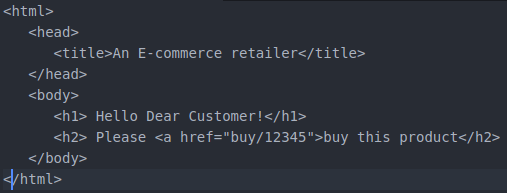
\includegraphics[scale=.7]{code1}
	\caption{insert caption}
\end{figure}

The Intrinsic Cognitive Load of this markup includes an understanding of the syntax and semantics of HTML, the ability to read the English language, and the knowledge that there is another component referenced by a hyperlink that completes the purchasing process. The Germane Cognitive Load includes some semantic understanding of the intent of the application--such as knowing that the 12345 corresponds to a product identifier that is used by another page to trigger purchasing. The Extraneous Cognitive Load includes the lack of an ending close tag for the anchor- -\textless/a\textgreater. Someone reading this document later may have difficulty understanding whether the intent was to only make the word “buy” a hyperlink, or whether the intention was to “buy this product.”

Suppose market research discovers that more purchases occur if the greeting is warm and friendly. The product team asks the development team to change the greeting to a formulation that has been shown to lead to more purchases, addressing the customer as “Dear, dear customer.” The development team has design options. They may implement the change by simply changing the text, as shown below:

\begin{figure}[H]
	\centering
	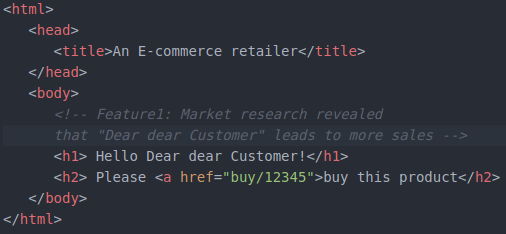
\includegraphics[scale=.7]{code2}
	\caption{insert caption}
\end{figure}

This simple change adds another word to the document, but has minimal effect on the intrinsic, germane, or extraneous cognitive load. A comment has been added to clarify why this changed.

Suppose further market research reveals that “Dear dear Customer” works well for people who shop with their browser set to the Spanish language, but “Valued Shopper” works better for others. The Intrinsic Cognitive Load of this application will increase. Either different pages will need to be loaded by the HTTP server based upon the customer’s location, or the markup will need to be updated in a way that enables the greeting to be displayed dynamically. The development team may choose the second option and generate the code below:

\begin{figure}[H]
	\centering
	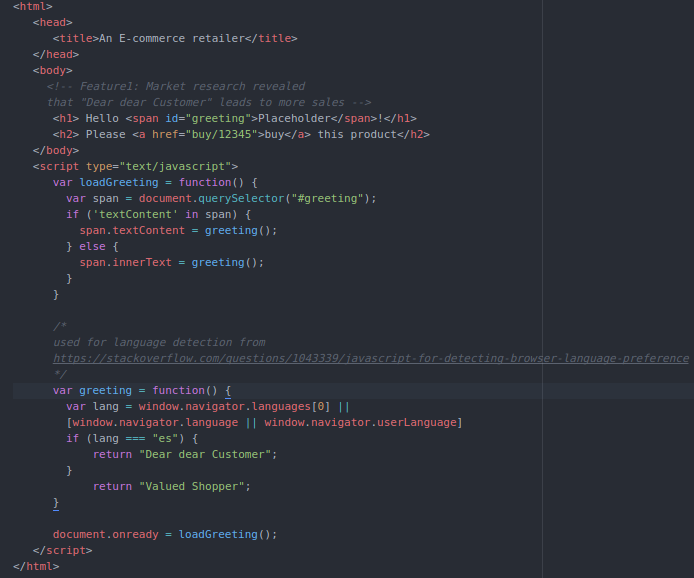
\includegraphics[width=\linewidth]{code3}
	\caption{insert caption}
\end{figure}

Not only has the Intrinsic Cognitive Load of this application increased conceptually, but the Cognitive Load imposed by the code has increased dramatically as well. A dynamic element has been introduced to the document through the use of Javascript, which will replace the HTML \textless span\textgreater with an id of “greeting” rendered text based on the detected value of the language when the document is ready. The Germane Cognitive Load now includes an understanding of Javascript language syntax, semantics, and eventing model, localization issues of language, and the platform-specific nuances of different browsers. The comment that was helpful in the static “simple” update is now Extraneous Cognitive Load, because what is rendered is no longer just “Dear dear Customer”, it may also be “Valued Shopper.” Future developers may question whether the code is correct because the comment tells them it should do one thing, but the code itself does another.

The Intrinsic Cognitive Load of the application cannot be reduced without changing its functionality. This Cognitive Load can be managed by sequencing and chunking. An enterprising developer may refactor the application as show below:

\begin{figure}[H]
	\centering
	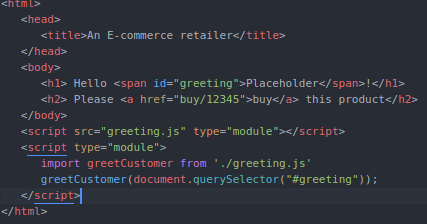
\includegraphics[scale=.7]{code4}
	\caption{insert caption}
\end{figure}

\begin{figure}[H]
	\centering
	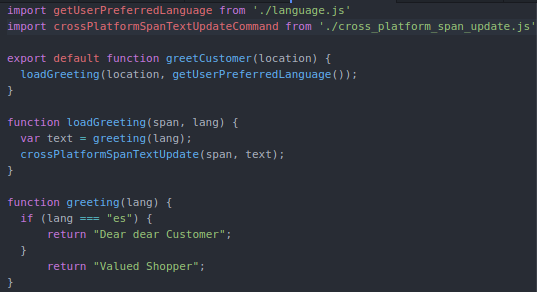
\includegraphics[scale=.7]{code5}
	\caption{insert caption}
\end{figure}

\begin{figure}[H]
	\centering
	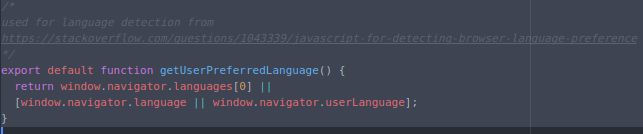
\includegraphics[width=\linewidth]{code6}
	\caption{insert caption}
\end{figure}

\begin{figure}[H]
	\centering
	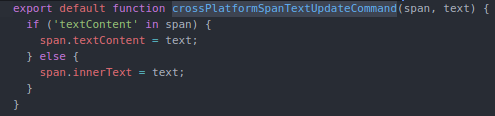
\includegraphics[scale=.7]{code7}
	\caption{insert caption}
\end{figure}

This refactoring introduces the concepts of sequencing and chunking. It adds Germane Cognitive Load by using JavaScript’s modules functionality, but the complexity of the original HTML file is dramatically reduced as its bits are chunked across multiple files, meant to be read and understood sequentially.
I propose the following hypotheses as links between software craftsmanship practices and CLT:
\begin{itemize}
	\item The Single Responsibility Principle is a technique that reduces Extraneous Cognitive Load and manages the Intrinsic Cognitive Load of classes by promoting smaller classes. In the above example, the single responsibility of the HTML page is to invoke the greetCustomer function.
	\item The Open/Closed Principle helps beginners manage Germane Cognitive Load by enabling consumers of classes to leverage existing components while avoiding cognitive overload by abstracting away inner details. In the above example, getUserPreferredLanguage is a default function whose implementation is closed to modification, but communicates intention through its name.
	\item The Newspaper Metaphor is a technique for minimizing the Split Attention Effect, reducing Extraneous Cognitive Load. In the above example, methods are arranged according to their usage.
	\item Design Patterns form a higher-level vocabulary that increases Germane Cognitive Load for intermediate/advanced developers, allowing richer conversations with less distracting detail. In the above example, the COMMAND pattern is used to convey that a function has a void return type and performs a side-effect.
	\item Smaller functions/methods with descriptive names align closely with Miller’s Magic Number Seven Plus or Minus Two [58], allowing programmers to hold more of a method’s functionality in their heads at once. This reduces context switching and makes the overall component easier to understand. This pattern scales. Small methods, small classes, small packages, small libraries, small frameworks are more cognitively available for novices, enabling quicker, less error-prone development. In the above example, none of the functions have more than 7 lines.
\end{itemize}

\section{Theory \& Predictions}

Cognitive Load Theory has shown measurable and repeatable results that have influenced Instructional Design. Refactoring patterns are widely accepted for reducing technical debt and making code easier to understand and modify, but it is hard to quantify this effect. In some software engineering companies, the process of peer code review is used as a mechanism for quality control and to manage technical debt. In code review discussions, the application of certain Refactoring techniques or the order in which they are applied can give rise to disagreements that they are simply about style versus substance. Someone without previous background in patterns literature may argue that the introduction of a pattern makes code more complicated. Sometimes one with such a background may argue that the wrong pattern is being applied.  Decision points about whether a block of code should become a separate method or class, the names of identifiers, the control structures leveraged, and other points of the software design and implementation can become a horse trading affair where software engineers try to persuade each other based on appeals to authority, tribal knowledge, and individual preference. Cognitive Load Theory offers a structured approach for measuring and quantifying the technical debt of a software project, and a conceptual framework to guide these discussions. Software teams can apply a practice of periodically reviewing certain classes in their code-base and subjectively reporting the estimated cognitive load. Such a practice would allow, over time, to use the measured change in reported cognitive load as a metric to include in the calculation of the technical debt of a project. 

Additionally, CLT guidelines can change the way we think about documenting and understanding code. For instance, an application of the Modality Effect suggests that embedding UML diagrams directly in source code that involves spatial reasoning, and providing audio narration could improve the comprehensibility of the code. Integrated Developer Environments  such as Eclipse Juno, IntelliJ IDEA 2014 and Visual Studio 2010 don’t support this type of experience natively. The guidelines of worked examples and self-explanations can provide a cognitive basis for the efficacy of Test/Behavior Driven Development. Guidelines related to separating system components from processes and supporting knowledge from procedure steps can inform arguments behind the viability of Interface Oriented Design \cite{Pugh2006} and the choices behind particular abstractions.

The complexity of software most often becomes an issue when the code has to change. The primary drivers of change in software are finding a defect or desiring a new feature. When the code must be changed, there is a risk that previous correct behavior may become incorrect, or that the performance profile--in terms of CPU utilization, memory usage, IO, or other factors-- may change in a dramatic way that affects the availability of the system. This is when the technical debt associated with the system may cause the necessary change to take hours, weeks, or more. If Cognitive Load Theory can quantify the technical debt a system experiences effectively, one would expect to find that systems with high technical debt impose high cognitive load on their maintainers and users. These high technical debt systems would contain more design flaws, more implementation bugs, and changes to these systems would take longer to implement and validate, hence being more likely to introduce regressions from desired behavior. Conversely, systems with lower technical debt should impose lower cognitive load. The number of design flaws and implementation defects should be lower, the average time to resolve issues should be less, and changes should introduce fewer regressions. Consequently, code that is refactored to manage its cognitive load more effectively should be code where one can more easily fix an outstanding bug, the attempt at fixing should introduce less regressions on average, and the engineers who attempt the fix should report less perceived cognitive load from the code they read and modify. A useful experiment would look at an existing piece of software with well-defined functionality and a known bug, create a refactored version that maintains the presence of the bug but more effectively manages the cognitive load, then verify that it is easier to fix the refactored version and that engineers feel less cognitive load while trying.

\section{Research Question: Can Cognitive Load Theory provide empirical evidence and a conceptual framework for the efficacy of Refactoring?}

The non-directional null-hypotheses to test, in mathematical terms, are:
\begin{enumerate}
	\item Time of completion (control) = Time of completion (refactored)
	\item Perceived Cognitive Load (control) = Perceived Cognitive Load (refactored)
	\item Average defects introduced (control) = average defects introduced (refactored)
\end{enumerate}

These hypotheses should be testable with a 95\% (p \textless .05) confidence level and desired power of 80\% ($\pi$=0.80).

\subsection{Why will this be meaningful?}

One would expect to find the code refactored to manage cognitive load requires less average time to fix defects and introduces less regressions while trying. This will enable the research community to explore further interventions and evaluate questions such as “do some principles have a higher impact when applied than others?”, “is the effect of the principles in any way tied to programming language?”, and “could results be affected familiarity with program domain?” Additionally, showing the efficacy of Cognitive Load Theory’s application to software engineering creates a wealth of opportunities to explore its recommendations for visualizations, organization of project documentation, and personalized tooling support for software engineer of various skill levels.

\subsection{What could go wrong?}

It is possible that authors wildly misrepresent the effects of the programming heuristics. Consequently, divergent results upon measurement may be unlike previous Cognitive Load experiments. Perhaps even with classical techniques of measuring Cognitive Load one will be unable to find a relationship between programming performance and Cognitive Load optimization techniques. This would suggest CLT is not as strong a fit for software as the original hypotheses suppose.  Additionally, Cognitive Load Theory states the principle of the Expertise Reversal Effect, which says that some practices that highly benefit novices will flummox experts and vice-versa. A robust experiment should identify instances of this by targeting an equal mix of novice and expert participants. One would expect that content increases Germane Cognitive Load, such as the lexicon of Design Patterns, would improve the performance of intermediate and proficient practitioners but may induce cognitive overload—and hence have a negative impact—on novice performance. Alternately, partitioning methods and classes to minimize the risk of cognitive overload may be unnecessary for an expert. Such efforts may improve novice performance, but inhibit the analysis of an expert who can “hold more of the code in their head.”  

\subsection{How can one measure the Cognitive Load of code?}

The Cognitive Load Theory literature describes multiple different options for measuring cognitive load. Paas et al provide a useful literature review \cite{Paas2003} that surveys analytical and empirical methods such as subjective rating, physiological response, and concurrent-task assessment. In separate work, Paas et al compared subjective ratings with psychophysiological response readings and found that subjective rating is reliable and sensitive enough to be useful without the significant cost and implementation barriers that come with more technological measurement \cite{Paas1994}. Brunken included direct forms of cognitive load measurement such as EEG \cite{Brunken2003} and found that a dual-task method may work well for multimedia. Given that the introduction and measurement of CLT are new when it comes to software, I chose a subjective rating scale where participants numerically rank items based on perceived difficulty--commonly known as a 7-point Likert Scale [93]-- to measure the induced cognitive load of code snippets.
       
With these conditions in mind, the next section presents the experiment that tested these hypotheses.
